% v2-acmtog-sample.tex, dated March 7 2012
% This is a sample file for ACM Transactions on Graphics
%
% Compilation using 'acmtog.cls' - version 1.2 (March 2012), Aptara Inc.
% (c) 2010 Association for Computing Machinery (ACM)
%
% Questions/Suggestions/Feedback should be addressed to => "acmtexsupport@aptaracorp.com".
% Users can also go through the FAQs available on the journal's submission webpage.
%
% Steps to compile: latex, bibtex, latex latex
%
% For tracking purposes => this is v1.2 - March 2012
\documentclass{acmtog} % V1.2

%\acmVolume{VV}
%\acmNumber{N}
%\acmYear{YYYY}
%\acmMonth{Month}
%\acmArticleNum{XXX}
%\acmdoi{10.1145/XXXXXXX.YYYYYYY}

\let\oldquote\quote
\let\endoldquote\endquote
\renewenvironment{quote}[2][]
  {\if\relax\detokenize{#1}\relax
     \def\quoteauthor{#2}%
   \else
     \def\quoteauthor{#2~---~#1}%
   \fi
   \oldquote}
  {\par\nobreak\smallskip\hfill(\quoteauthor)%
   \endoldquote\addvspace{\bigskipamount}}

\acmVolume{1}
\acmNumber{1}
\acmYear{2018}
\acmMonth{March}
\acmArticleNum{1}
%\acmdoi{10.1145/1559755.1559763}
\makeatletter
\def\runningfoot{\def\@runningfoot{}}
\def\firstfoot{\def\@firstfoot{}}
\makeatother



\begin{document}

\markboth{Experimental Sentiment Analysis on Twitter}{A Real Time Stream and Big Data Process}

\title{Sentiment Analysis on Twitter : Effects of a Social Network} % title

\author{Mohamed Ben Hamdoune {\upshape and} Yannis Tannier
\affil{University of Paris-Descartes}
% NOTE! Affiliations placed here should be for the institution where the
%       BULK of the research was done. If the author has gone to a new
%       institution, before publication, the (above) affiliation should NOT be changed.
%       The authors 'current' address may be given in the "Author's addresses:" block (below).
%       So for example, Mr. Fogarty, the bulk of the research was done at UIUC, and he is
%       currently affiliated with NASA.
}

\category{I.3.7}{Database}{Big Data and Real Stream}[Cloud Computing]
\category{I.3.5}{Social Media Analytics}{Apache Spark and Hadoop}[Machine Learning]

\terms{Twitter, Psychological Profil}

\keywords{Natural Languages Processing, Contradiction Analysis, Opinon Mining, Classification, Text Mining}

\acmformat{Mohamed Ben Hamdoune, Yannis Tannier. 2018. Sentiment Analysis for Twitter : Effect of a Social Network.}

\maketitle

\begin{bottomstuff}
Jason Scott Sadofsky acknowledges a Jason Scott, is an American archivist, historian of technology, and filmmaker. Archive Team is a group dedicated to preserving digital history that was founded by Jason Scott in 2009. Data was collected from the website of The Archive Team.
\end{bottomstuff}


\begin{abstract}
Our purpose is to build a powerful platform for real-time data analysis of tweets on twitter trends. We also want to analyse all the tweets of 2017 based on a downloaded sample of data (average of 6To). All this data analysis will be accessible via a web interface that will be developed. We want to build a powerful system of sentiments analysis by making a database structure of tweets which is relevant about impacts and effects. The system should provide a faster way to execute Machine Learning methodologies behind data extracted from Twitter. Analysis news actuality by getting an analysis on actual trends with real stream data by building an efficient web interface to get results easily and build a system without false accounts and keep a control on data continuously.
\end{abstract}

\section{Introduction}
The main subject is Sentiment Analysis on Twitter, a microblogging platform where people can easily share their thought on anything and their habits too. We have a lot of publications on sentiment analysis but not so much research about impacts and their effect on society. The maximum characters are 140 which can be a good thing for the process of analysis because it will make it faster in a way to perform on small messages but in the other hand we should pay attention on accuracy of results. Event it’s an enormously continuous stream of data, Twitter is a good extra sentiment though an online community. Therefore, how to optimize all those streaming data and build a web interface for users who want to get data. Our project will use many methodologies from Machine Learning like unsupervised methods to make a classification of sentiments, and supervised method to predicate psychological profile. Finally, one big step will be and efficient system about control of massive data incoming, a check on false account and spam messages that will destroy our results for example.
 
\begin{quote}{Jeffrey Zeldman}
“The best way to engage honestly with the marketplace via Twitter is to never use the words "engage," "honesty," or "marketplace." 
\end{quote}

In this study, we introduce readers to the problems of Data Processing and Cloud Computation, which have been rapidly developing over the last decade. The rest of this document is organized as follows. In Sect. 2, we provide a specific view of Tweet format. Development, problems, definitions and main trends of this area are described in Sect 3. We analyze in Sect 6, and discuss in Sect 7 about several problems we have been through.
Finally, we talk about others idea and features that were not implemented due to a lack of time in Sect 8.

\section{Related Work}
\label{sec:related_work}

To begin, ye can refer to this article [cite palpatine] because we can relate that it is a point of start, it gives us a theoretical review on the development of Sentiment Analysis.
The interested reader can also refer to previous surveys in the area, like [cite] and [cite], that helped us on machine learning techniques. As an active research field that has emerged for a long time now, sentiment analysis is now been greatly implement but it is also with a cost (for example, IBM Watson Tone Analyzer). Sentiment analysis is a discipline that extracts people’s feelings, opinions, thoughts and behaviors from user’s text data using Natural Language Processing (NLP) methods. 
For methodologies on preprocessing, and feature generation, we based our work on [deep learning]. Then we can also cite [chinois publication] for a reason, they removed numbers from theirs tweet thinking that in general, numbers are of no use when measuring sentiment and are removed from tweets to refine the tweet content but we wanted to keep them thinking the contrary.
Based on 36 million tweets collected from Twitter, Wang et al. proposed a real-time sentiment analysis system for classification of political tweets during 2012 US presidential elections. Their model achieved 59% accuracy in predicting the sentiments of political tweets (Wang et al., 2012).
We had over 800 million tweets in English and all that data to analyze where possible just because of the MapReduce Model [cite les grecs] in majority.


The data for this task consists of tweets across various domains, classified into four emotions : joy, sadness, anger and fear. The training data additionally carries a real-valued score between 0 and 1 per tweet, indicating the degree of the emotion (that the tweet is classified as) the present in the tweet.
A very quick presentation of all steps in the project:
\begin{enumerate}
\item Fetch data with API (main language we will use is Python), manage collections of stream data.
\item Pre-processing on data with Spark.
\item Build multiple module.
\item Analysis those data with multiple methods of machine learning.
\item Web interface.
\end{enumerate}

\section{Methodology}
\label{sec:methodology}

blabla

\subsection{Preprocessing (Data clean)}
\label{subsub:preprocessing}

blabla

\subsection{Feature Generation}
\label{subsub:feature}

The data for this task consists of tweets across various domains, classified into four emotions: joy, sadness, anger and fear. The training data additionally carries a real-valued score between 0 and 1 per tweet, indicating the degree of the emotion (that the tweet is classified as) the present in the tweet.

\section{Cloud Computing}
\label{sec:cloud_computing}

Cloud computing was used for the project, the trend today is machine learning, which is a form of artificial intelligence that uses algorithms to learn from data. These systems build models from incoming transactional data, then find patterns in that data to make predictions. These predictions can be a simple as providing a recommendation to a shopper on an e-commerce website or as complex as determining if a brand of automobile should be retired. As with their learning-system forebears, the overhead of machine-learning systems is typically huge. But today we have the option to place these systems in the cloud. Amazon Web Services, for example, supports machine learning using AWS's algorithms to read native AWS data (such as RDS, Redshift, and S3). Google has supported predictive analysts for some time with its Google Prediction API, and Microsoft provides an Azure machine-learning service. The ability to predict the future for both tactical and strategic purposes has eluded us because of prohibitive resource requirements. But today, thanks to the cloud for machine learning as a service, you can apply this technology far and wide on all that data enterprises have been collecting.

\subsection{AWS (Amazon Web Service)}
\label{subsub:aws}

blabla

\subsection{MapReduce Model and Spark Framework}
\label{subsub:mapreduce_spark}

blabla

\subsection{Conception of the Database for the Web Interface}
\label{subsub:conception}

The World Wide Web (Web, for short), is a distributed information system based on hypertext. Web interfaces to databases have become very important. After outlining several reasons for interfacing databases with the Web, we provide an overview of Web Technology. We then outline techniques for building Web interfaces to databases.


\section{Implementation}
\label{sec:implementation}

\We have used the following technologies for many reasons. Hadoop assumes that conventional approaches (consisting of developing ever more powerful centralized systems) have technical and financial limitations. The development of distributed systems consisting of machines or nodes, relatively affordable (commodity hardware) and scaling out is an alternative from a technical and financial point of view A distributed system comprising tens, hundreds or thousands of nodes will regularly be confronted with hardware and / or software failures. Google has developed the Google File System (GFS), ancestor of the Hadoop Disrelated File System (HDFS) and The MapReduce Approach. MapReduce is a programming model designed specifically to read, milk and write very large volumes of data. A Hadoop program usually implements both map tasks and reduce tasks.
Hadoop is particularly effective for dealing with problems that have one or more of the following characteristics: Volume of data to store or process very important. Need to perform processing on all data (batch rather than transactional, therefore). Heterogeneous data in terms of origin, structure, and format (JSON) Execute the tasks of a Hadoop job in parallel, without a pre-established order. A Hadoop cluster is made up of tens, hundreds, or thousands of nodes. It is the addition of the storage and processing capacities of each of these nodes which makes it possible to offer a storage space and a computing power yet to handle data volumes of several To or Po. To improve the performance of a read / write cluster, Hadoop’s file management system, HDFS, writes and reads files in blocks of 64 MB or 128 MB. Working on such large blocks maximizes data transfer rates by limiting search time on hard drives (seek time). // Input file graph and block MapReduce is a programming model designed specifically to read, process and write very large volumes of data. A Hadoop program usually implements both map tasks and reduce tasks. A Hadoop program is usually divided into three parts: The driver, which runs on a client machine, is responsible for configuring the job and submitting it for execution. The map is responsible for reading and processing data stored on disk. The reducer is responsible for consolidating the results from the map and write them on disk.

\section{Results}
\label{sub:results}

\begin{figure*}[t]
\centerline{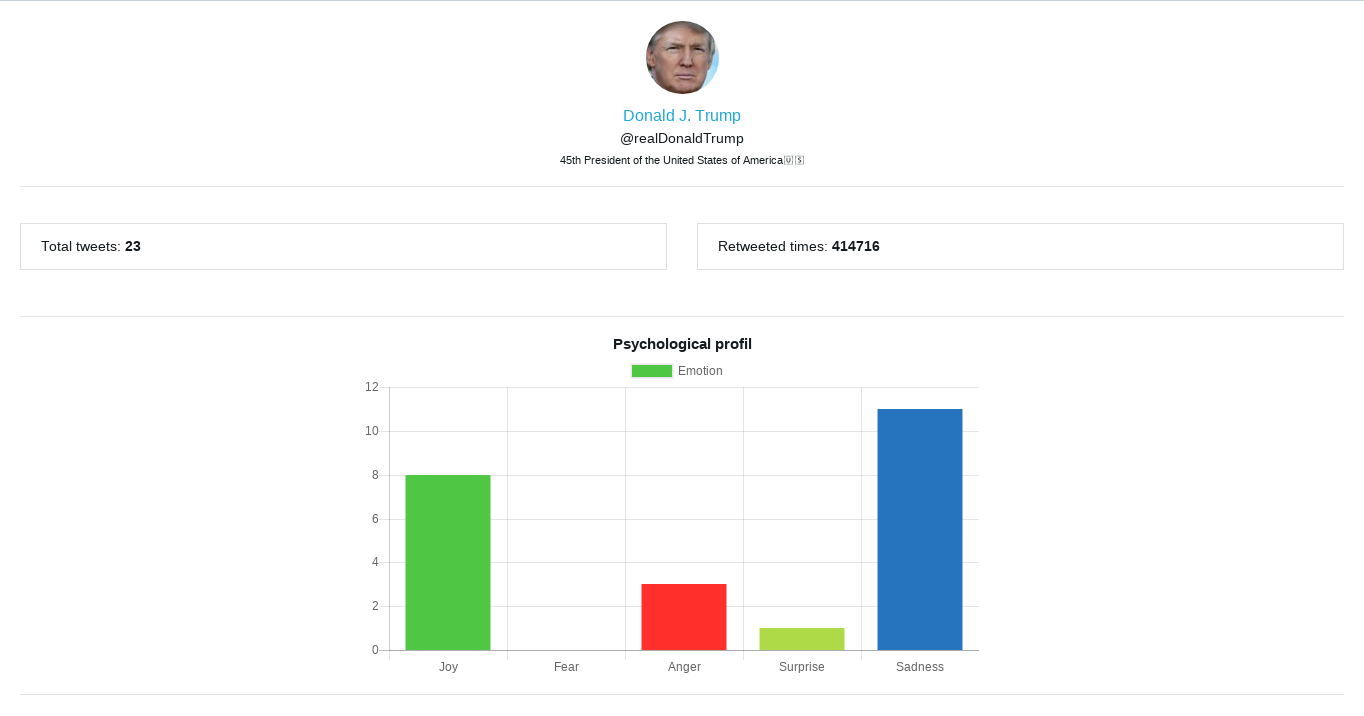
\includegraphics[height=0.5\textwidth]{trump.png}}
\caption{Results predicted by our models with Donald John Trump (born June 14, 1946), the 45th and current President of the United States.}
  \label{fig:trump_results}
\end{figure*}

\section{Analysis}
\label{sec:analysis}
We have used the following technologies for a number of reasons. Hadoop assumes that conventional approaches (consisting of developing ever more powerful centralized systems) have technical and financial limitations.
The development of distributed systems consisting of machines or nodes, relatively affordable (commodity hardware) and scaling out is an alternative from a technical and financial point of view
A distributed system comprising tens, hundreds or thousands of nodes will regularly be confronted with hardware and / or software failures.
Google has developed the Google File System (GFS), ancestor of the Hadoop Disreated File System (HDFS) and The MapReduce Approach.
MapReduce is a programming model designed specifically to read, milk and write very large volumes of data. A Hadoop program usually implements both map tasks and reduce tasks.

Hadoop is particularly effective for dealing with problems that have one or more of the following characteristics:
Volume of data to store or process very important.
Need to perform processing on all data (batch rather than transactional, therefore).
Heterogeneous data in terms of origin, structure, and format (JSON)
Execute the tasks of a Hadoop job in parallel, without a pre-established order.
A Hadoop cluster is made up of tens, hundreds, or thousands of nodes. It is the addition of the storage and processing capacities of each of these nodes which makes it possible to offer a storage space and a computing power yet to handle data volumes of several To or Po.
To improve the performance of a read / write cluster, Hadoop's file management system, HDFS, writes and reads files in blocks of 64 MB or 128 MB. Working on such large blocks maximizes data transfer rates by limiting search time on hard drives (seek time).
// Input file graph and block
MapReduce is a programming model designed specifically to read, process and write very large volumes of data. A Hadoop program usually implements both map tasks and reduce tasks.
A Hadoop program is usually divided into three parts:
The driver, which runs on a client machine, is responsible for configuring the job and submitting it for execution.
The map is responsible for reading and processing data stored on disk.
The reducer is responsible for consolidating the results from the map and write them on disk.

\section{Discussion}
\label{sec:results}

Hence, the difference between Apache Storm vs Spark Streaming shows that Apache Storm is a solution for real-time stream processing. But Storm is very complex for developers to develop applications. There are very limited resources available in the market for it.
Storm can solve only one type of problem i.e Stream processing. But the industry needs a generalized solution which can solve all the types of problems. For example Batch processing, stream processing interactive processing as well as iterative processing. Here Apache Spark comes into limelight which is a general purpose computation engine. It can handle any type of problem. Apart from this Apache Spark is much too easy for developers and can integrate very well with Hadoop.

Apache Spark is an in-memory distributed data analysis platform-- primarily targeted at speeding up batch analysis jobs, iterative machine learning jobs, interactive query and graph processing.
One of Spark's primary distinctions is its use of RDDs or Resilient Distributed Datasets. RDDs are great for pipelining parallel operators for computation and are, by definition, immutable, which allows Spark a unique form of fault tolerance based on lineage information. If you are interested in, for example, executing a Hadoop MapReduce job much faster, Spark is a great option (although memory requirements must be considered).
Apache Storm is focused on stream processing or what some call complex event processing. Storm implements a fault tolerant method for performing a computation or pipelining multiple computations on an event as it flows into a system. One might use Storm to transform unstructured data as it flows into a system into a desired format.
Storm and Spark are focused on fairly different use cases. The more "apples-to-apples" comparison would be between Storm Trident and Spark Streaming. Since Spark's RDDs are inherently immutable, Spark Streaming implements a method for "batching" incoming updates in user-defined time intervals that get transformed into their own RDDs. Spark's parallel operators can then perform computations on these RDDs. This is different from Storm which deals with each event individually.
One key difference between these two technologies is that Spark performs Data-Parallel computationswhile Storm performs Task-Parallel computations. Either design makes tradeoffs that are worth knowing. I would suggest checking out these links.

\section{Conclusion}
\label{sec:conclusion}
%
We have presented new models for realistic renderings of the human iris
and pupil. Our physiologically-based model of the pupil light reflex
combines and extends theoretical results from the Mathematical Biology
field with experimental data collected by several researchers. The
resulting model is expressed in terms of a nonlinear delay-differential
equation that describes the changes in the pupil diameter as function of
the environment lighting. Our model is also original in the sense that
it can simulate individual differences with respect to light
sensitivity. As all parameters of our models were derived from
experimental data, they correctly simulate the actual behavior of the
human iris and pupil. They also produce high-fidelity appearance
effects, which can be used to create\break real-time predictive
animations of the pupil and iris under variable lighting conditions. We
have validated our models through comparisons of our simulated results
against videos and photographs captured from human irises. The quality
of these simulations qualitatively matched the actual behaviors of human
pupils and irises.

To the best of our knowledge, ours is the first physiologically-based
model for simulating pupil light reflex presented in the graphics
literature. It is also the first practical model (providing actual
coefficient values) in the literature for simulating the dynamics of
pupil and iris under variable lighting conditions, and the first
integrated model in all of the literature to consider individual
variability in pupil diameter using general equations for latency and
velocity. Our image-based model for iridal pattern deformation is also
the first model of its kind in the graphics literature.\vskip21pt

% Start of "Sample References" section
\section{References}

\begin{acks}
We are grateful to the following people for resources,discussions and suggestions: Jason Scott(Archivist),Diana Yuan (Co-Founder & Vice President, Talent & Operations from Indico).
\end{acks}


% Bibliography
\bibliographystyle{ACM-Reference-Format-Journals}
\bibliography{publication-bibfile}

                                % Sample .bib file with references that match those in
                                % the 'Specifications Document (V1.5)' as well containing
                                % 'legacy' bibs and bibs with 'alternate codings'.
                                % Gerry Murray - March 2012

\end{document}
% End of v2-acmtog-sample.tex (March 2012) - Gerry Murray, ACM
